\documentclass[
  11pt,
  letterpaper,
  % addpoints,
   answers
  ]{exam}
\usepackage{float}
\usepackage{../exercise-preamble}

\begin{document}

\noindent
\begin{minipage}{0.47\textwidth}
  
\includegraphics[width=\textwidth]{../fcfm_die}
\end{minipage}
\begin{minipage}{0.53\textwidth}
\begin{center} 
\large\textbf{Electromagnetismo Aplicado} (EL3103) \\
\large\textbf{Clase auxiliar 4} \\
\normalsize Prof.~\professor\\
\normalsize Prof. Aux. Lucas Palomino
\\
\normalsize Ayudantes: \ayudanteA~-~\ayudanteB
\end{center}
\end{minipage}

\vspace{0.5cm}
\noindent
\vspace{.85cm}
\section{Resumen:}
\subsection*{Método de diferencias finitas (FDM)}
\begin{itemize}
    \item Cuando tenemos una ecuación de Laplace o de Poisson que entrega EDOs o EDPs muy complicadas, podemos resolver mediante el método de diferencias finitas, que permite transformar a un sistema lineal de ecuaciones.
    \item Para esto, discretizamos un cuerpo continuo haciendo una malla, y podemos obtener el potencial en diversos puntos dependiendo de cómo construyamos la malla.
    \item El único requerimiento es \textbf{conocer el potencial en una frontera.}
\end{itemize}
\subsection*{Desarrollo del método para un material cargado ($\rho \neq 0$)}
Si tenemos una malla del estilo:

\vspace{0.5cm}
\begin{center}

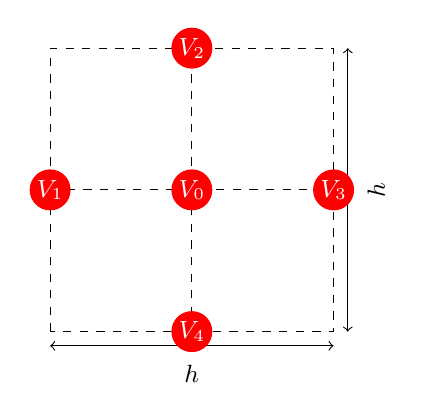
\begin{tikzpicture}[scale=1.2, every node/.style={font=\small}]

\def\h{1.5} % tamaño de la celda

% Cuadrado de la celda (líneas punteadas)
\draw[dashed] (-\h,0) -- (\h,0);
\draw[dashed] (0,-\h) -- (0,\h);
\draw[dashed] (-\h,-\h) rectangle (\h,\h);

% Distancias h
\draw[<->] (-\h,-1.1*\h) -- (\h,-1.1*\h);
\node at (0,-1.3*\h) {$h$};

\draw[<->] (1.1*\h,-\h) -- (1.1*\h,\h);
\node[rotate=90] at (1.3*\h,0) {$h$};

% Nodos vecinos (rojos)
\filldraw[red] (0,\h) circle (6pt);
\node[text=white] at (0,\h) {$V_2$};

\filldraw[red] (-\h,0) circle (6pt);
\node[text=white] at (-\h,0) {$V_1$};

\filldraw[red] (\h,0) circle (6pt);
\node[text=white] at (\h,0) {$V_3$};

\filldraw[red] (0,-\h) circle (6pt);
\node[text=white] at (0,-\h) {$V_4$};

% Nodo central (rojo)
\filldraw[red] (0,0) circle (6pt);
\node[text=white] at (0,0) {$V_0$};


\end{tikzpicture}
\captionof{figure}{Malla para cálculo de potencial en cada punto de esta, usando valores de puntos cercanos.}
\label{fig:malla_FDM}
\end{center}
\vspace{0.3cm}
Para resolver en torno a $V_0$, se establece la ecuación de diferencias finitas (\textit{five-point equal arm difference}) como:
\begin{align}
    \frac{1}{h^2}(V_1 + V_2 + V_3 + V_4 - 4V_0) &= - \frac{\rho}{\epsilon_0}
\end{align}
\subsubsection*{Caso para un único material no cargado:}
Si tenemos una malla como la de la figura \ref{fig:malla_FDM}, entonces el potencial al centro de esta ($V_0$) se puede calcular por la siguiente fórmula:
\begin{align}
    V_0 \approx \frac{1}{4}(V_1 + V_2 + V_3 + V_4)
\end{align}
Esto viene de que $\rho = 0$, por ende, se simplifica la fórmula.

\subsection*{Caso para dos dieléctricos (no cargados):}
Con una malla del estilo:

\begin{center}
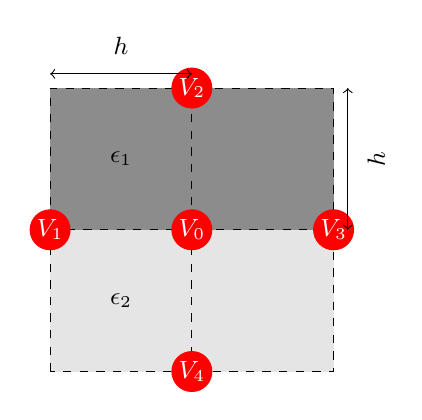
\begin{tikzpicture}[scale=1.2, every node/.style={font=\small}]
\def\h{1.5} % mitad del lado (el lado del cuadro es 2h)

% --- RELLENOS (primero, para no tapar líneas/texto) ---
\fill[gray!90] (-\h,0) rectangle (0,\h);   % región superior izquierda: eps1
\fill[gray!20] (-\h,-\h) rectangle (0,0);  % región inferior izquierda: eps2
\fill[gray!90] (0,0) rectangle (\h,\h);    % sup. derecha (solo estética)
\fill[gray!20] (0,-\h) rectangle (\h,0);   % inf. derecha (solo estética)

% --- LÍNEAS PUNTEADAS (borde y divisiones) ---
\draw[dashed] (-\h,-\h) rectangle (\h,\h);
\draw[dashed] (-\h,0) -- (\h,0);          % horizontal
\draw[dashed] (0,-\h) -- (0,\h);          % vertical

% --- ETIQUETAS DE PERMITIVIDAD ---
\node at (-0.5*\h,  0.5*\h) {$\epsilon_1$};
\node at (-0.5*\h, -0.5*\h) {$\epsilon_2$};

% --- NODOS (rojos) ---
\filldraw[red] (0,0) circle (6pt) node[text=white] {$V_0$};
\filldraw[red] (-\h,0) circle (6pt) node[text=white] {$V_1$};
\filldraw[red] (0,\h) circle (6pt) node[text=white] {$V_2$};
\filldraw[red] (\h,0) circle (6pt) node[text=white] {$V_3$};
\filldraw[red] (0,-\h) circle (6pt) node[text=white] {$V_4$};

% --- FLECHAS h ---
\draw[<->] (-\h,1.1*\h) -- (0,1.1*\h);        \node at (-0.5*\h,1.3*\h) {$h$};
\draw[<->] (1.1*\h,0) -- (1.1*\h,\h);         \node[rotate=90] at (1.3*\h,0.5*\h) {$h$};

\end{tikzpicture}
\captionof{figure}{Malla para cálculo de potencial entre dos dieléctricos.}
\end{center}
Si queremos el potencial en un punto en la interfaz (en este caso sería $V_0$), la fórmula es la siguiente:
\begin{align}
    V_0 \approx \frac{1}{2(\epsilon_1 + \epsilon_2)} \left[ \frac{1}{2} (\epsilon_1 + \epsilon_2) V_1+ V_2 \epsilon_1 + \frac{1}{2} (\epsilon_1 + \epsilon_2)V_3 + V_4 \epsilon_2 \right]
\end{align}
\textit{Observación: Si tuviéramos un solo medio, se recupera la ecuación} (2).

\subsection*{Diferencias finitas centradas (central-difference)}
Para calcular derivadas en un punto $(x_0, y_0)$, utilizaremos valores cercanos para hacer la siguiente aproximación:
\begin{align}
    \frac{\partial f}{\partial x} & \approx \frac{f(x_0 + h_x) - f(x_0 - h_x)}{2 \cdot h_x} \\
    \frac{\partial f}{\partial y} & \approx \frac{f(y_0 + h_y) - f(y_0 - h_y)}{2 \cdot h_y}
\end{align}
La ventaja de esta aproximación es que tiene un error del orden $O(h^2)$ (si reducimos el valor de $h$ a la mitad, el error se reduce a un cuarto). Es decir, si tomamos un valor de $h$ lo suficientemente bajo, el error es despreciable. 
\newpage
\section{Ejercicios:}
\begin{questions}
  
\question \label{q: FDM_1} Una placa de un material con constantes $\epsilon, \mu$ posee dimensiones de $\qty{8}{\centi\m}\times\qty{8}{\centi\m}$, y se le aplica potencial como muestra \cref{fig: FDM_f1}. Entonces, determine el potencial en el centro de la placa y el campo eléctrico en el centro de la placa. 

\vspace{0.5cm}
\begin{center}
    
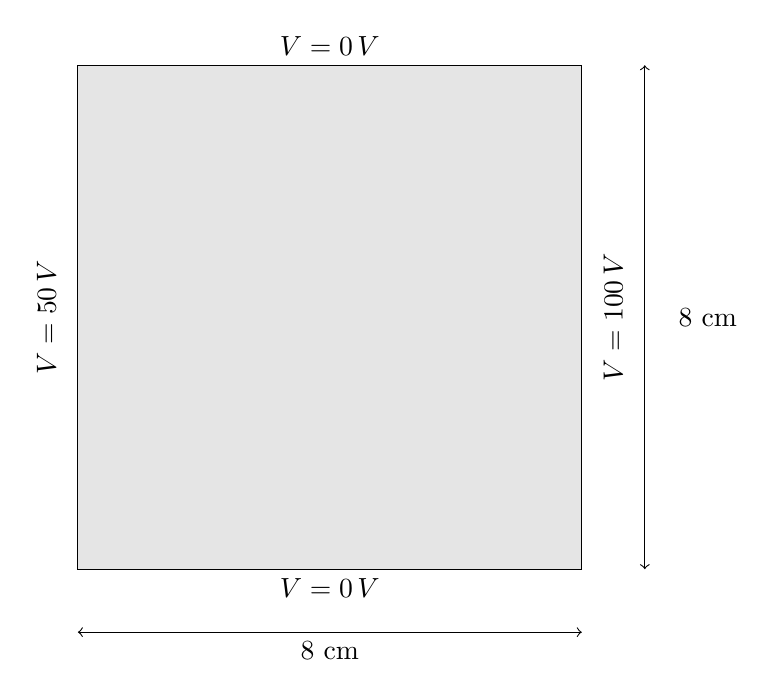
\begin{tikzpicture}[scale=0.8]

% Cuadrado
\draw[fill=gray!20] (0,0) rectangle (8,8);

% Etiquetas de potencial
\node at (4,8.3) {$V = 0 \, \text{V}$};
\node[rotate=90] at (-0.5,4) {$V = 50 \, \text{V}$};
\node at (4,-0.3) {$V = 0 \, \text{V}$};
\node[rotate=90] at (8.5,4) {$V = 100 \, \text{V}$};

% Dimensiones horizontales
\draw[<->] (0,-1) -- (8,-1);
\node at (4,-1.3) {8 cm};

% Dimensiones verticales
\draw[<->] (9,0) -- (9,8);
\node at (10,4) {8 cm};
    
\end{tikzpicture}
\captionof{figure}{Placa con potencial.}
\label{fig: FDM_f1}
\end{center}
\begin{solution}
Buscamos una discretización tal que tenga un nodo al centro del cuadrado. 

\vspace{0.4cm}
\begin{center}

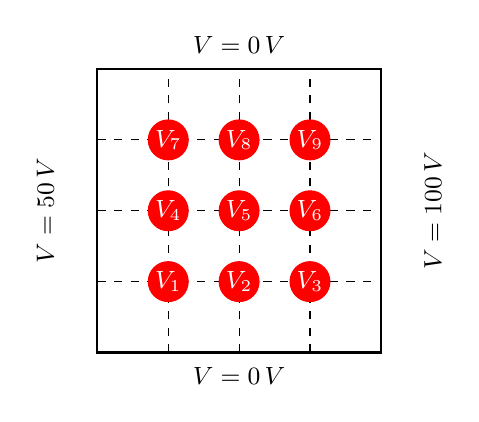
\begin{tikzpicture}[scale=1.2, every node/.style={font=\small}]
\def\L{3}   % lado del cuadrado
\def\n{3}   % cantidad de nodos interiores por eje (3x3)
\pgfmathsetmacro{\step}{\L/(\n+1)} % = 3/4 = 0.75

% Marco
\draw[thick] (0,0) rectangle (\L,\L);

% Condiciones de borde
\node at (0.5*\L, \L+0.25) {$V=0\,\text{V}$};
\node[rotate=90] at (-0.55, 0.5*\L) {$V=50\,\text{V}$};
\node[rotate=90] at (\L+0.55, 0.5*\L) {$V=100\,\text{V}$};
\node at (0.5*\L, -0.25) {$V=0\,\text{V}$};

% Líneas de malla (internas)
\foreach \i in {1,...,\n} {
  \draw[dashed] (\i*\step,0) -- (\i*\step,\L);
  \draw[dashed] (0,\i*\step) -- (\L,\i*\step);
}

% Nodos interiores 3x3, V1..V9
\foreach \j in {1,...,\n}{
  \foreach \i in {1,...,\n}{
    \pgfmathtruncatemacro{\idx}{(\j-1)*\n + \i}
    \filldraw[red] (\i*\step,\j*\step) circle (6pt);
    \node[text=white] at (\i*\step,\j*\step) {$V_{\idx}$};
  }
}
\end{tikzpicture}
\captionof{figure}{Malla para la pregunta \ref{q: FDM_1}, donde cada cuadrado tiene dimensiones $h=2 cm$.}
\end{center}
De esta manera, como tenemos una placa no cargada y donde hay un único medio, utilizaremos la ecuación $V_0 = \frac{1}{4}(V_1 + V_2 + V_3 + V_4)$ para cada nodo y obtendremos el siguiente sistema de ecuaciones:
\begin{align}
    V_1 &= \frac{1}{4}(50 + 0 + V_2 + V_4) \rightarrow 4V_1 - V_2 - V_4 = 50 \\
    V_2 &= \frac{1}{4}(V_1 + 0 + V_3 + V_5) \rightarrow 4V_2 -V_1 -V_3 - V_5 = 0\\
    V_3 &= \frac{1}{4}(100 + 0 + V_6 + V_2) \rightarrow 4V_3 - V_6 - V_2 = 100 \\
    V_4 &= \frac{1}{4}(50 + V_1 + V_5 + V_7) \rightarrow 4V_4 - V_1 - V_5 - V_7 = 50 \\
    V_5 &= \frac{1}{4}(V_2 + V_4 + V_6 + V_8) \rightarrow 4V_5 - V_2 - V_4 - V_6 - V_8 = 0 \\
    V_6 &= \frac{1}{4}(100 + V_3 + V_9 + V_5) \rightarrow 4V_6 - V_3- V_5 - V_9 = 100\\
    V_7 &= \frac{1}{4}(50 + 0 + V_4 + V_8) \rightarrow 4 V_7 - V_4 - V_8 = 50\\
    V_8 &= \frac{1}{4}(0 + V_5 + V_7 + V_9) \rightarrow 4V_8 - V_5 - V_7 - V_9 = 0 \\
    V_9 &= \frac{1}{4}(0 + 100 + V_6 + V_8) \rightarrow 4V_9 - V_6 - V_8 = 100 \\
\end{align}
Pasando a sistema matricial:
\begin{align}
    \begin{bmatrix}
        4 & -1 & 0 & -1 & 0 & 0 & 0 & 0 & 0 \\
        -1 & 4 & -1 & 0 & -1 & 0 & 0 & 0 & 0 \\
        0 & -1 & 4 & 0 & 0 & -1 & 0 & 0 & 0 \\
        -1 & 0 & 0 & 4 & -1 & 0 & -1 & 0 & 0 \\
        0 & -1 & 0 & -1 & 4 & -1 & 0 & -1 & 0 \\
        0 & 0 & -1 & 0 & -1 & 4 & 0 & 0 & -1 \\
        0 & 0 & 0 & -1 & 0 & 0 & 4 & -1 & 0 \\
        0 & 0 & 0 & 0 & -1 & 0 & -1 & 4 & -1 \\
        0 & 0 & 0 & 0 & 0 & -1 & 0 & -1 & 4 \\
    \end{bmatrix}
    \cdot \begin{bmatrix}
        V_1 \\
        V_2 \\
        V_3 \\
        V_4 \\
        V_5 \\
        V_6 \\
        V_7 \\
        V_8 \\
        V_9 \\
    \end{bmatrix}
    =
    \begin{bmatrix}
        50 \\
        0 \\
        100 \\
        50 \\
        0 \\
        100 \\
        50 \\
        0 \\
        100
    \end{bmatrix}
\end{align}
\textit{Observación: Ya con dejar el sistema matricial expresado tenemos la distribución del potencial. Pero nos piden el potencial al centro de la placa, y al ser una matriz de 9x9, es muy difícil resolver este sistema a mano. Es por eso que podemos usar una propiedad de la ecuación de Laplace que dice que el potencial al centro será el promedio de los extremos. De esta forma:}

\begin{align}
    V_5 &= \frac{0 + 100 + 0 + 50}{4} = 37,5 [V]
\end{align}
Es lo mismo que obtendríamos al resolver el sistema matricial, pero nos ahorramos el desarrollo. Eso si, \textbf{en el control DEBEN utilizar el método de diferencias finitas hasta llegar a la matriz, recién ahí pueden usar la propiedad de la ecuación de Laplace.} 
\\
\\
Ahora debemos obtener el campo al centro de la placa. Para esto, utilizamos que:
\begin{align}
    \mathbf{E} &= - \nabla V \\
    \mathbf{E} &= - \frac{\partial V}{\partial x} \hat{x}- \frac{\partial V}{\partial y} \hat{y}
\end{align}
Para calcular estas derivadas, usamos diferencias finitas centradas (\textit{central-difference}), es decir: 
\begin{align}
    \frac{d V}{dx} & \approx \frac{V(x_5 + h) - V(x_5 - h)}{2h} = \frac{V_6 - V_4}{2 \cdot 2} = \frac{V_6 - V_4}{4} \\
    \frac{d V}{dy} & \approx \frac{V(x_5 + h) - V(x_5 - h)}{2h} = \frac{V_8 - V_2}{2 \cdot 2} = \frac{V_8 - V_2}{4}
\end{align}
De esta forma, el campo en el centro de la placa es:
\begin{align}
    \mathbf{E} &= \frac{V_4 - V_6}{4} \hat{x} + \frac{V_2 - V_8}{4} \hat{y}
\end{align}
\end{solution}

\question \label{q: FDM_2} Se tiene un material compuesto de dos medios con permitividades $\epsilon_1$ y $\epsilon_2$, como se muestra en la \cref{fig: fdm_f2}. Se requiere calcular una distribución para el potencial a través de todo el material tal que esta tenga puntos en la interfaz.
\vspace{0.3cm}
  \begin{center}
    \begin{tikzpicture}
      \def\L{3cm};
      \coordinate (A) at (-\L, \L);
      \coordinate (B) at (0, \L);
      \coordinate (C) at (\L, \L);
      \coordinate (D) at (-\L, 0);
      \coordinate (E) at (0, 0);
      \coordinate (F) at (\L, 0);
      \coordinate (G) at (-\L, -\L);
      \coordinate (H) at (0, -\L);
      \coordinate (I) at (\L, -\L);


      \draw[very thick] (C) rectangle (G);
      \path[top color=gray!200,bottom color=gray!100,shading angle=-20] (A) -- (C) -- (F) -- (D) -- cycle;

      \path[top color=gray!20,bottom color=gray!50,shading angle=20] (G) -- (I) -- (F) -- (D) -- cycle;

      \node[gray!200] at (-\L/2, -\L/2) {$\epsilon_2$};
      \node[gray!20] at (-\L/2, \L/2) {\color{white}$\epsilon_1$};

      % \foreach \i in {A, B, C, D, E, ..., I}{
      %   \node[fill=white] at (\i) {\i};
      % }

      % potentials
      \node[below, rotate=90] at (F) {$V = \qty{0}{\volt}$};
      \node[above] at (B) {$V = \qty{50}{\volt}$};
      \node[below] at (H) {$V = \qty{35}{\volt}$};
      \node[above, rotate=90] at (D) {$V=\qty{0}{\volt}$};

      \draw[|<->|] ($(C) + (1, 0)$) -- ($(I) + (1, 0)$) node[rotate=90,midway, fill=white] {\qty{10}{\centi\m}};
      \draw[|<->|] ($(A) + (0, 1)$) -- ($(C) + (0, 1)$) node[midway, fill=white] {\qty{10}{\centi\m}};

    \end{tikzpicture}
    \captionof{figure}{Material compuesto de dos medios, \cref{q: FDM_2}.}
    \label{fig: fdm_f2}
  \end{center}
\begin{solution}
    Cuando nos pidan una distribución para el potencial, basta con dejar expresado el sistema matricial. Es importante darse cuenta que utilizaremos la ecuación (3) solo en la interfaz. Para el resto de casos, utilizamos la ecuación (2). De esta forma, establecemos la malla más simple posible y que tenga puntos en la interfaz:

    \begin{center}
      \begin{tikzpicture}
        \def\L{3cm};
        \coordinate (A) at (-\L, \L);
        \coordinate (B) at (0, \L);
        \coordinate (C) at (\L, \L);
        \coordinate (D) at (-\L, 0);
        \coordinate (E) at (0, 0);
        \coordinate (F) at (\L, 0);
        \coordinate (G) at (-\L, -\L);
        \coordinate (H) at (0, -\L);
        \coordinate (I) at (\L, -\L);
  
  
        \draw[very thick] (C) rectangle (G);
        \path[top color=gray!150,bottom color=gray!50,shading angle=-20] (A) -- (C) -- (F) -- (D) -- cycle;
  
        \path[top color=gray!10,bottom color=gray!40,shading angle=20] (G) -- (I) -- (F) -- (D) -- cycle;
  
        % \foreach \i in {A, B, C, D, E, ..., I}{
        %   \node[fill=white] at (\i) {\i};
        % }
  
        % potentials
        \node[below, rotate=90] at (F) {$V = \qty{0}{\volt}$};
        \node[above] at (B) {$V = \qty{50}{\volt}$};
        \node[below] at (H) {$V = \qty{35}{\volt}$};
        \node[above, rotate=90] at (D) {$V=\qty{0}{\volt}$};

        \draw[|<->|] (C) ++ (.5, 0) -- ++ (0, -\L/2) node[midway, fill=white] {$h$};
        \draw[|<->|] ($(B)!.5!(C)$) ++ (0, .5) -- ++ (\L/2, 0) node[midway, fill=white] {$h$};
  

        % node coordinates
        \coordinate (nA) at (-\L/2, \L/2);
        \coordinate (nB) at (0, \L/2);
        \coordinate (nC) at (\L/2, \L/2);
        \coordinate (nD) at (-\L/2, 0);
        \coordinate (nE) at (0, 0);
        \coordinate (nF) at (\L/2, 0);
        \coordinate (nG) at (-\L/2, -\L/2);
        \coordinate (nH) at (0, -\L/2);
        \coordinate (nI) at (\L/2, -\L/2);

        \path[draw, dashed, thin] ($(A)!.5!(D)$) -- ($(C)!.5!(F)$);
        \path[draw, dashed, thin] (D) -- (F);
        \path[draw, dashed, thin] ($(D)!.5!(G)$) -- ($(F)!.5!(I)$);
        \path[draw, dashed, thin] ($(A)!.5!(B)$) -- ($(G)!.5!(H)$);
        \path[draw, dashed, thin] (B) -- (H);
        \path[draw, dashed, thin] ($(B)!.5!(C)$) -- ($(H)!.5!(I)$);


        \foreach \x/\y in {nI/9, nH/8, nG/7, nF/6, nE/5, nD/4, nC/3, nB/2, nA/1}{
          \node[draw, white, circle, fill=red, inner sep=0pt] at (\x) {$V_\y$};
        }
        
        \node[gray!20] at ($(A)!.5!(nA)$) {\color{white}$\epsilon_1$};
        \node[gray!200] at ($(G)!.5!(nG)$) {$\epsilon_2$};
  
      \end{tikzpicture}
      \captionof{figure}{Malla para la \cref{q: FDM_2}.}
      \label{fig:fdm_sol}
    \end{center}
  Entonces desarrollamos para nodos $V_1$--$V_9$ y obtenemos:
    \begin{align}
      V_1 &= \frac{1}{4}\del{V_4 + V_2 + \num{50}} \\
      V_2 &= \frac{1}{4}\del{V_1 + V_5 + V_3 + \num{50}} \\
      V_3 &= \frac{1}{4}\del{V_2 + V_6 + \num{50}} \\
      V_4 &= \frac{1}{2\del{\epsilon_1 + \epsilon_2}} \sbr{\epsilon_1V_1 + \frac{1}{2}\del{\epsilon_1 + \epsilon_2}V_5 + \epsilon_2V_7} \\
      V_5 &= \frac{1}{2\del{\epsilon_1 + \epsilon_2}} \sbr{\epsilon_1V_2 + \frac{1}{2}\del{\epsilon_1 + \epsilon_2}\del{V_4 + V_6} + \epsilon_2V_8} \\
      V_6 &= \frac{1}{2\del{\epsilon_1 + \epsilon_2}} \sbr{\epsilon_1V_3 + \frac{1}{2}\del{\epsilon_1 + \epsilon_2}V_5 + \epsilon_2V_9} \\
      V_7 &= \frac{1}{4}\del{V_4 + V_8 + \num{35}} \\
      V_8 &= \frac{1}{4}\del{V_7 + V_5 + V_9 + \num{35}} \\
      V_9 &= \frac{1}{4}\del{V_8 + V_6 + \num{35}}.
    \end{align}
    Resolviendo el sistema de ecuaciones obtenemos:
    \begin{align}
      \sbr{\begin{matrix}
         -4 & 1 & 0 & 1 & 0 & 0 & 0 & 0 & 0 \\
          1 & -4 & 1 & 0 & 1 & 0 & 0 & 0 & 0 \\
          0 & 1 & -4 & 0 & 0 & 1 & 0 & 0 & 0 \\
          \epsilon_1 & 0 & 0 & -2\del{\epsilon_1 + \epsilon_2} & \frac{1}{2}\del{\epsilon_1 + \epsilon_2} & 0 & \epsilon_2 & 0 & 0 \\
          0 & \epsilon_1 & 0 & \frac{1}{2}\del{\epsilon_1 + \epsilon_2} & -2\del{\epsilon_1 + \epsilon_2} & \frac{1}{2}\del{\epsilon_1 + \epsilon_2} & 0 & \epsilon_2 & 0 \\
          0 & 0 & \epsilon_1 & 0 & \frac{1}{2}\del{\epsilon_1 + \epsilon_2} & -2\del{\epsilon_1 + \epsilon_2} & 0 & 0 & \epsilon_2 \\
          0 & 0 & 0 & 1 & 0 & 0 & -4 & 1 & 0 \\
          0 & 0 & 0 & 0 & 1 & 0 & 1 & -4 & 1 \\
          0 & 0 & 0 & 0 & 0 & 1 & 0 & 1 & -4
      \end{matrix}} 
      \sbr{\begin{matrix}
        V_1 \\ V_2 \\ V_3 \\ V_4 \\ V_5 \\ V_6 \\ V_7 \\ V_8 \\ V_9
        \end{matrix}} &=
        \sbr{\begin{matrix}
          -\num{50} \\ 0 \\ -\num{50} \\ 0 \\ 0 \\ 0 \\ -\num{35} \\ 0 \\ -\num{35}
        \end{matrix}}. 
    \end{align}
Y de esta forma obtenemos la distribución pedida.
  \end{solution}

\question \label{q: FDM_3} Se tiene una región rectangular de $\qty{6}{\m} \times \qty{8}{\m}$, donde el potencial es exactamente igual a cero en sus cuatro fronteras. La distribución de carga, sin embargo, está dada por $\rho = 2\epsilon_0$. 
\begin{parts}
    \part Resuelva numéricamente la ecuación de Poisson definiendo una ecuación de potencial (i.e., \textit{five-point equal arm difference}) y determine la distribución del potencial en la región rectangular.
    \part \textbf{[Propuesto]} Obtenga el campo eléctrico para todos los puntos de la discretización.
\end{parts}
\begin{solution}
\begin{parts}
 \part Ahora tendremos que usar la ecuación five-point equal arm difference completa, es decir, la ecuación (1) del resumen. Notemos que la distribución de carga $\rho$ es igual a $2 \epsilon_0$, de esta forma, la expersión $-\frac{\rho}{\epsilon_0}$ queda igual a $-\frac{2 \epsilon_0}{\epsilon_0} = -2$. Usamos la siguiente discretización:
    \begin{center}
      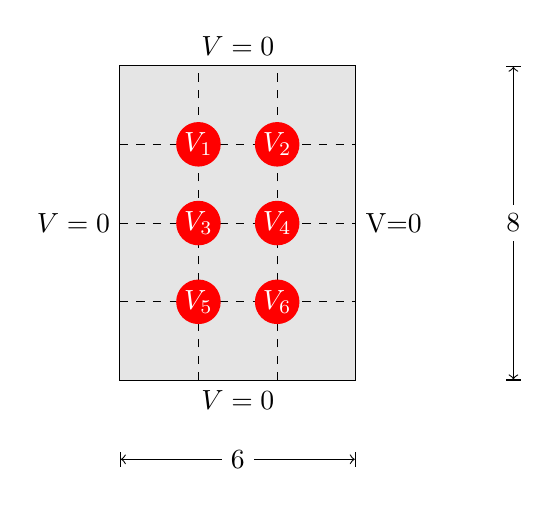
\begin{tikzpicture}[scale=.5]
  
        \edef\width{6}
        \edef\height{8}
        \edef\h{2}

        \draw[fill=gray!20] (0, 0) coordinate (A) -- ++ (\width, 0) coordinate (B) node[midway, below] {$V=\qty{0}{\volt}$} -- ++ (0, \height) coordinate (C) node[midway, right] {V=\qty{0}{\volt}} -- ++ (-\width, 0) coordinate (D) node[midway, above] {$V=\qty{0}{\volt}$} -- cycle node[midway, left] {$V=\qty{0}{\volt}$};

        \foreach \x in {1, 2}{
          \draw[dashed] ({\x*\h}, 0) -- ({\x*\h}, \height);
        }
        \foreach \y in {1, 2, 3}{
          \draw[dashed] (0, {\y*\h}) -- (\width, {\y*\h});
        }

        \node[white, circle, fill=red, inner sep=1pt] at ({1*\h}, {1*\h}) {$V_5$};
        \node[white, circle, fill=red, inner sep=1pt] at ({1*\h}, {2*\h}) {$V_3$};
        \node[white, circle, fill=red, inner sep=1pt] at ({1*\h}, {3*\h}) {$V_1$};
        \node[white, circle, fill=red, inner sep=1pt] at ({2*\h}, {1*\h}) {$V_6$};
        \node[white, circle, fill=red, inner sep=1pt] at ({2*\h}, {2*\h}) {$V_4$};
        \node[white, circle, fill=red, inner sep=1pt] at ({2*\h}, {3*\h}) {$V_2$};

        \draw[|<->|] (A) ++ (0, -2) -- ++ (\width, 0) node[midway, fill=white] {
          \qty{6}{\m}
        };
        \draw[|<->|] (B) ++ (4, 0) -- ++ (0, \height) node[midway, fill=white] {
          \qty{8}{\m}
        };
      \end{tikzpicture}
      \captionof{figure}{Resolución \cref{q: FDM_3}}
      \label{fig:dfm}
    \end{center}
    Y utilizamos la siguiente ecuación para cada punto:
    \begin{equation}
      \frac{1}{h^2}\del{V_{i+1, j} + V_{i+1, j} + V_{i, j+1} + V_{i, j-1}, 4V_{i, j}} = -\frac{\rho}{\epsilon_0} = -2, \label{eq:five-point}
    \end{equation}
    con $h$ el tamaño del elemento usado. Dividimos entonces usando $h=\qty{2}{\m}$, y el sistema matricial queda:
    \begin{equation}
      \sbr{
      \begin{array}{cccccc}
        -4 & 1 & 1 & 0 & 0 & 0 \\
        1 & -4 & 0 & 1 & 0 & 0 \\
        1 & 0 & -4 & 1 & 1 & 0 \\
        0 & 1 & 1 & -4 & 0 & 1 \\
        0 & 0 & 1 & 0 & -4 & 1 \\
        0 & 0 & 0 & 1 & 1 & -4 \\
      \end{array}} \sbr{\begin{array}{c} V_1 \\ V_2 \\ V_3 \\ V_4 \\ V_5 \\ V_6 \end{array}} =\sbr{\begin{array}{c} -8 \\ -8 \\ -8 \\ -8 \\ -8 \\ -8\end{array}}.
    \end{equation}
    Podemos invertir la matriz o directamente calcular las ecuaciones, que por simetría son:
    \begin{equation}
      V_1 = V_2 = V_5 = V_6, \qquad \text{y} \qquad V_3 = V_4,
    \end{equation}
    luego $V_1 = \qty{4.56}{\volt}$ y $V_3=\qty{5.72}{\volt}$.
    \end{parts}
\end{solution}
\end{questions}
 \end{document}